\chapter{Marco técnico}

\section{Ruby}

\emph{Ruby} \cite{ruby} es un lenguaje de programación interpretado, reflexivo, orientado a objetos y de código abierto creado por el programador japonés Yukihiro ``Matz'' Matsumoto, quien comenzó a trabajar en él en 1993, y lo presentó públicamente en 1995. Combina una sintaxis inspirada en Python y Perl con características de programación orientada a objetos similares a Smalltalk. Comparte también funcionalidad con otros lenguajes de programación como Lisp, Lua, Dylan y CLU. 

\emph{Ruby} ha sido descrito como un lenguaje de programación multiparadigma: permite programación procedural (definiendo funciones y variables fuera de las clases haciéndolas parte del objeto raíz Object), con orientación a objetos, (todo es un objeto) o funcionalmente (tiene funciones anónimas, clausuras o closures, y continuations; todas las sentencias tienen valores, y las funciones devuelven la última evaluación). Soporta introspección, reflexión y metaprogramación, además de soporte para hilos de ejecución gestionados por el intérprete. \emph{Ruby} tiene tipado dinámico, y soporta polimorfismo de tipos (permite tratar a subclases utilizando la interfaz de la clase padre).

\section{Ruby on Rails}
\emph{Ruby on Rails} \cite{rubyonrails}, es un framework para desarrollo de aplicaciones web de código abierto escrito en el lenguaje de programación \emph{Ruby}, siguiendo el paradigma de la arquitectura Modelo Vista Controlador (MVC). Fue diseñado para hacer la programación de aplicaciones web más simple, tratando de combinar la simplicidad con la posibilidad de desarrollar aplicaciones del mundo real escribiendo menos código que con otros frameworks y lenguajes de programación y manteniendo también un mínimo de configuración. El lenguaje de programación \emph{Ruby} permite la metaprogramación, de la cual Rails hace uso, lo que resulta en una sintaxis que muchos de sus usuarios encuentran muy legible.
\emph{Rails} supone que existe una ``mejor'' forma de hacer las cosas y está diseñado para fomentar al programador a hacerlas de esa forma, intentando así un aumento en la productividad.
La filosofía de \emph{Rails} fomenta los siguientes principios:
\begin{itemize}
\item
\textbf{DRY} El principio DRY (``Don't Repeat Yourself'' o ``No te repitas a ti mismo'') indica que es una buena práctica evitar repetir código de manera innecesaria.
\item
\textbf{Convención sobre configuración} implica que el desarrollador sólo debe especificar aspectos no convencionales de la aplicación. Rails propone un conjunto de convenciones a seguir que facilitan el desarrollo y permiten evitar tener archivos de configuración.

\end{itemize}

\subsection{Gemfile}

El archivo Gemfile.rb es el  lugar donde se listan las dependencias (gemas) de un proyecto \emph{Ruby on Rails}. En el mismo se debe incluir el nombre de la gema y es opcional incluir la
versión de la misma que se desea utilizar. Para instalar las mismas es necesario tener instalado \emph{bundler}. Una vez disponible este comando, instalar las dependencias es tan 
sencillo como ejecutar el siguiente comando desde una terminal \emph{bundle install}.

\subsection{La arquitectura MVC}
En el núcleo de \emph{Rails} se encuentra la arquitectura Modelo-Vista-Controlador (MVC). Algunos de los beneficios que brinda la arquitectura MVC incluyen la separación de la lógica de negocio de la interfaz, facilita el mantenimiento del código DRY, indica claramente dónde ubicar diferentes tipos de código para facilitar posteriormente el mantenimiento de la aplicación.
\subsubsection{Modelos}
Un modelo representa la información de la aplicación y las reglas para manejar esos datos. En el caso de \emph{Rails} los modelos son utilizados principalmente para manejar las reglas de interacción con la tabla correspondiente en una base de datos. En la mayoría de los casos, cada tabla en la base de datos se corresponderá a un modelo en la aplicación. La mayor cantidad de lógica de negocio de la aplicación debería concentrarse en los modelos.
\subsubsection{Vistas}
Las vistas representan la interfaz de usuario de la aplicación. En \emph{Rails}, las vistas son habitualmente archivos HTML con código \emph{Ruby} embebido que realiza únicamente tareas relacionadas con la presentación de los datos. Las vistas manejan el trabajo de proveer información al navegador o la herramienta utilizada para hacer pedidos desde la aplicación.
\subsubsection{Controladores}
Los controladores realizan la unión entre modelos y vistas. En \emph{Rails}, los controladores son responsables de procesar los pedidos provenientes del navegador, realizando los pedidos necesarios a los modelos para obtener la información y pasarla a las vistas para que sea presentada.

\subsection{Backbone}

Backbone.js \cite{backbone} es una librería Javascript que permite implementar el patrón de desarrollo MVC (Modelo-Vista-Controlador) del lado del cliente. \emph{Backbone} brinda estructura al 
código Javascript al proveer modelos con asociaciones del tipo clave-valor, colecciones y vistas con manejo declarativo de eventos, y permite conectar todo esto con el 
\emph{backend} mediante una interfaz \emph{JSON RESTful}.

Los Modelos de \emph{Backbone} pueden ser creados, validados, destruidos y enviados al servidor para persistirlos. Cuando una acción en la interfaz de 
usuario genera un cambio en un atributo del modelo,  éste último dispara un evento de cambio.  Las vistas encargadas de desplegar el estado del modelo pueden ser notificadas de 
este cambio, responder de manera acorde, y volver a \emph{renderizarse} con la nueva información.


\section{Facilidades de Ruby on Rails para cumplir con las reglas de performance}

En esta sección se desarrolla un resumen de cómo \emph{Ruby on Rails} brinda mecanismos y herramientas para poder cumplir con las reglas de performance de forma sencilla y transparente al desarrollador web. Por cada regla relevante se brindará una descripción de lo que ofrece el framework para cumplirla.

\subsection{Realizar menos pedidos HTTP}

Como fue descrito en secciones anteriores, existen varias formas de reducir la cantidad de pedidos necesarios por parte del cliente para cargar un sitio. La mayoría de los
pedidos realizados para lograrlo, son recursos de tipo imagen, hojas de estilo (CSS) y \emph{scripts} (Javascript).

Como ya se detalló en secciones anteriores, uno de los problemas existentes es tener muchos archivos separados de hojas de estilo y \emph{scripts}. Esto genera que el navegador
del usuario deba realizar un pedido por cada uno de los recursos. Sin embargo, tener estos archivos separados favorece la mantenibilidad debido a la modularización, basándose en la
idea de ``divide y vencerás''. De ser necesario unificar todos los archivos en uno, se perderían las características anteriormente mencionadas, tornando el desarrollo más complejo.

Para resolver este problema, a partir de su versión 3.1.0, \emph{Ruby on Rails} brinda un componente llamado \emph{asset pipeline}.  La idea detrás del mismo, es resolver el
problema de unificación de recursos, sin perder las características deseables de practicidad en el desarrollo. Dado el mantra convención sobre configuración, si un desarrollador
sigue las convenciones del \emph{asset pipeline}, obtendrá automáticamente los dos beneficios buscados. Para ello, todos los recursos anteriormente mencionados deberán
estructurarse en la aplicación de la siguiente forma:

\begin{figure}[h]
\centering
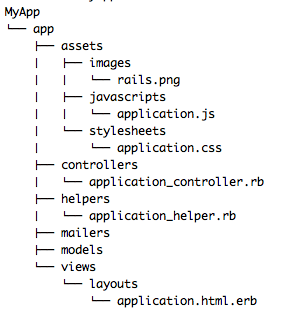
\includegraphics[width=0.5\textwidth]{figuras/rails_app.png}
	\caption{Estructura de aplicación rails típica}
    \label{fig.aplicacion_rails_tipica}
\end{figure}

Dentro del directorio \emph{app/assets} de una aplicación \emph{Rails} típica (ver figura \ref{fig.aplicacion_rails_tipica}), existen por defecto tres directorios:
\emph{images}, \emph{styesheets} y \emph{javascripts}. Como indican sus nombres, el desarrollador deberá introducir los recursos de cada tipo en la carpeta correspondiente. Para
las hojas de estilo y los \emph{scripts} el desarrollador tiene a su disposición una serie de meta funciones que le permiten indicar dependencia entre archivos. Por ejemplo:
Supongamos que el desarrollador tiene dos archivos \emph{javascript}, \emph{principal.js} y \emph{modulo.js}. Para indicar que el archivo \emph{principal.js} requiere al archivo \emph{modulo.js}, dentro
del archivo \emph{principal} debe agregarse una línea con el siguiente contenido, ``//= require modulo''. Esto le indicará al \emph{asset pipeline} cuando realice la compilación de los
recursos, que dentro del archivo \emph{principal.js}, debe incluirse el contenido del archivo \emph{modulo.js}. 

La idea detrás de esto, es que el desarrollador incluya un único archivo de hojas
de estilo y de \emph{scripts} y que en ellos se incluya todo el código de aplicación necesario. Para incluir archivos unificados de recursos, el desarrollador solamente debe
utilizar los métodos que provee \emph{Rails}, \emph{javascript\_include\_tag(script)} y \emph{stylesheet \_link\_tag(hoja de estilo)} en el \emph{layout} más general de la aplicación. El
primer método genera un elemento HTML de tipo \emph{script} con el atributo \emph{src} igual a la ruta del archivo parámetro. El segundo genera un elemento HTML de tipo
\emph{a} con el atributo \emph{href} igual a la ruta de la hoja de estilos unificada.

El \emph{asset pipeline} soluciona este problema para las hojas de estilo y los \emph{scripts}, sin embargo, existe el mismo problema con las imágenes. A priori parecería que seguir
una solución del mismo estilo para las imágenes, no es muy intuitiva. Hay dos tipos de imágenes, las de naturaleza cambiante (por ejemplo, las generadas por usuarios en redes
sociales), y las que se mantienen estáticas en el tiempo, como por ejemplo iconos, logos de empresas, etc. 

Para las imágenes de naturaleza cambiante no hay mucho que hacer, ya
que generalmente no se tiene control sobre ellas. Para las imágenes estáticas existen diferentes técnicas para agruparlas, y que el navegador del usuario deba realizar menos
pedidos. Una de las técnicas ya mencionadas para realizar esta optimización es realizar \emph{CSS sprites}. La idea detrás de esta técnica es unificar las imágenes estáticas en una
única imagen, y que el navegador del usuario realice un único pedido. Luego, por medio de directivas \emph{CSS} desplegar fragmentos de la imagen unificada como si fueran
imágenes individuales.

\emph{Ruby on Rails} no incluye por defecto ningún mecanismo para utilizar esta técnica. Sin embargo, existen paquetes fáciles de incluir en la aplicación que hacen que implementar esta
técnica sea sencillo. Uno de los paquetes disponibles al día de hoy es \emph{compass} \cite{compass}. Para incluir esta dependencia en una aplicación
\emph{Rails}, hay que agregar la siguiente línea en el Gemfile ``gem rails-compass''. Éste paquete genera \emph{CSS sprites} a partir de carpetas de imágenes, realizando el proceso de
unificación de imágenes de manera automática. Además, genera una clase \emph{CSS} por cada imagen perteneciente al \emph{sprite}. Cada clase tiene asignada el atributo
\emph{background-image} a la imagen unificada generada y el atributo \emph{background-position} en el valor adecuado para desplegar la imagen que se encuentra dentro del \emph{sprite}.

Para indicarle a \emph{compass} qué carpeta se desea utilizar para generar el \emph{sprite} se deben agregar las siguientes líneas a la hoja de estilo de la aplicación:
\begin{itemize}

\item @import compass

\item @import 'icons/*.png', esta línea le indica a \emph{compass} que debe unificar en un \emph{sprite} todas las imágenes de tipo PNG dentro de la carpeta icons.

\item @include all-icons-sprites, esta línea le indica a \emph{compass} que debe incluir dentro de la hoja de estilo las clases \emph{CSS} generadas, para que el desarrollador haga uso de
ellas.
\end{itemize}

Por más que \emph{compass} brinde todas estas facilidades, convertir el HTML generado al necesario para utilizar los \emph{sprites} puede tornarse difícil, y puede volver el manejo
de imágenes a futuro un poco más complicado, sin embargo, si se trata de muchas imágenes, la mejora en la reducción de pedidos puede llegar a ser muy significativa.
En futuras secciones se verá la aplicación de \emph{compass} en un caso de estudio de la realidad.

%minificación
\subsection{Minificación}

Otra manera de mejorar la performance en aplicaciones web ligada a los recursos de tipo \emph{javascript} y hojas de estilo, es la minificación de los mismos.
\emph{Rails} otorga esta mejora a través del \emph{asset pipeline} de manera muy transparente, brindando algunas facilidades. Para mantener la comodidad durante el desarrollo,
en los archivos de tipo \emph{script} y hojas de estilo se utilizan espacios, tabulaciones y saltos de línea para mantener la claridad y mantenibilidad en el código. En el ambiente de
desarrollo el \emph{asset pipeline} no realiza minificación alguna, permitiendo que la depuración del código sea más accesible.

 En el ambiente de producción, se realiza la
minificación de estos archivos de manera automática, utilizando por defecto el compresor \emph{uglifier}. El minificador puede cambiarse de manera sencilla, simplemente incluyendo
su paquete en el Gemfile y cambiando la configuración del \emph{asset pipeline} para que lo utilice.

\subsection{Compresión}
\label{cap4:cumpl_rails:compresion}

Con respecto a la regla de compresión, el \emph{asset pipeline} en el ambiente de producción en el momento de compilación además de minificar los recursos, también los comprime
utilizando \emph{gzip}. Luego, es necesario configurar el servidor web para que entregue estos archivos cuando los navegadores realicen pedidos.
Los servidores web son capaces de comprimir los archivos exactamente antes de entregarlos. La facilidad que el \emph{asset pipeline} brinda es la de dejarlos comprimidos,
evitando el trabajo de compresión que de lo contrario hubiera sido necesario realizar por pedido.

\subsection{Expires y Renombrado de archivos}

Una forma de evitar que el navegador realice pedidos innecesarios es explotar al máximo el \emph{cache} del navegador. Para lograr esto, se debe configurar a los servidores web para que
retornen en las respuestas a los pedidos por los recursos el encabezado \emph{Expires}. El objetivo es enviar una fecha de expiración muy adelantada en el tiempo, por ejemplo un
año. Esto se debe a que una vez que el navegador realizó \emph{caching} sobre algún contenido, cada vez que se realice un pedido por dicho recurso, el navegador solo realizará
el pedido si el archivo no ha expirado, ahorrando una enorme cantidad de pedidos innecesarios.
 
El problema que puede surgir es que si el archivo es modificado en el servidor, no hay manera de invalidar el \emph{cache} del navegador, ya que el mismo utiliza
la URL del archivo para guardarlo. Solamente realizará el pedido por ese recurso nuevamente una vez que el mismo haya expirado en su \emph{cache}.
Mediante el \emph{asset pipeline} \emph{Rails} brinda un mecanismo para evitar este problema. 

En el proceso de compilación de los recursos, se calcula una clave md5 basada en el
contenido de cada recurso. A cada recurso se le agrega ésta clave md5 en su nombre de archivo. De esta manera, cuando se produce un cambio en un archivo, la clave md5
generada para el mismo también cambiará, resultando en un cambio en la URL de ese recurso. Este cambio produce que el navegador no sea capaz de detectar que se trata del
mismo archivo. 

Para el desarrollador, toda la complejidad del manejo de las URLs con claves md5 generadas en tiempo de compilación es completamente transparente. Lo
único que debe hacer es utilizar los métodos \emph{javascript\_include\_tag} y \emph{stylesheet\_link\_tag}, con la ruta a los archivos.

\subsection{Utilizar \emph{scripts} y hojas de estilo externas}

Tener el código \emph{javascript} y de hojas de estilo separado del código HTML tiene beneficios, como por ejemplo explotar al máximo el cache del navegador. Sin embargo, tener
muchos archivos externos separados por página, puede traer la desventaja de que el navegador deba realizar un pedido por cada recurso. Como ya se detalló, la convención de
\emph{Rails} lleva a que todos los recursos se unifiquen en un solo archivo por tipo de recurso. Esto explota la ventaja de recursos externos sin sufrir la penalidad de tener muchos
archivos separados.

\subsection{Configurar \emph{Etags}}

Como se indicó en secciones anteriores, el mecanismo de los \emph{Etags} funciona de la siguiente manera. Cuando el navegador realiza un pedido a una página o recurso, en la
respuesta del servidor se incluye un encabezado que identifica al contenido pedido. Este encabezado varía según la implementación del servidor web, por ejemplo en la
implementación de Apache, el \emph{etag} depende del número de i-nodo del recurso en el servidor.

 Uno de los problemas es que si se dispone de varios servidores, el número de inodo de
un mismo recurso varía de servidor a servidor con una probabilidad muy alta. Sin embargo, la implementación de los \emph{Etags} puede ser modificada a nivel de aplicación.
En el caso de los recursos de tipo \emph{script} y hojas de estilo, la convención en \emph{Rails} es deshabilitar los \emph{Etags} para aprovechar los mecanismos de claves md5 
descritos en secciones anteriores. En el caso de otros tipos de recursos como páginas generadas, \emph{Rails} devuelve como \emph{Etag} para dicho recurso, la clave md5 del 
contenido de la respuesta generada. Esta implementación no es susceptible al problema mencionado anteriormente, ya que el contenido del recurso no variará de servidor a servidor.

\begin{comment}
\section{Buenas prácticas}
En estas secciones se presentan buenas prácticas para el trabajo con javascript, css y el mejor aprovechamiento del cache del protocolo HTTP.

\chapter{Recomendaciones para mejorar la performance de Javascript}
Las aplicaciones web de la actualidad utilizan una gran cantidad de codigo Javascript, en particular algunas utlizan Javascript para ejecutar gran parte de la
interfaz de usuario. Como resultado se tienen varias lineas de código que se ejecutan cada vez que el usuario interactúa con la página. Por lo tanto la performance
no sólo involucra el tiempo en que tarda la página en cargar, sino también como responde la interfaz de usuario al ser utilizada.

\section{Scope}
Cuando se ejecuta código Javascript, se crea un contexto de ejecución (denominado \emph{scope}). El contexto de ejecución define el entorno en el cual el código es
ejecutado. Un contexto de ejecución global es creado al cargar la página, contextos adicionales son creados para cada función que se ejecuta, por lo que se crea
un \emph{stack} de contextos de ejecución, en el cual el que se encuentra al comienzo, es el contexto de ejecución activo.

Cada contexto de ejecución tiene una \emph{scope chain} asociada, que es utilizada para la resolución de identificadores. La \emph{scope chain} contiene uno o más
objetos que definen identificadores para el contexto de ejecución. El contexto de ejecución global tiene un sólo objeto variable en su \emph{scope chain}, el cual define
todas las variables globales y funciones disponibles en Javascript.

Cuando una función es creada pero no ejecutada, su propiedad interna [[Scope]] contiene la \emph{scope chain} del contexto de ejecución en el cual fue creada. En
cuanto el flujo de ejecución entra en una función, un ``objeto de activación'' es creado e inicializado con valores para \emph{this}, \emph{arguments}, \emph{named arguments}
y las variables locales correspondientes a la función. El objeto de activaciones ubicado al comienzo de la \emph{scope chain} del contexto de ejecución es seguido por
los objetos contenidos en la propiedad [[Scope]] de la función.

Durante la ejecución, los identificadores como los nombres de las funciones y variables son resueltos buscando en la \emph{scope chain} del contexto de ejecución. La resolución
de identificadores comienza al principio de la \emph{scope chain}. Consideremos el siguiente ejemplo de código:

\begin{em}
function add(num1, num2)\{
    return num1 + num2;
\}

var result = add(5, 10);
\end{em}

Cuando éste código es ejecutado, la función add tiene una propiedad [[Scope]] que solo contiene al objeto global. En el momento en que el flujo de ejecución entra en la función
suma, un nuevo contexto de ejecución es creado, y un objeto de activación, conteniendo \emph{this}, \emph{arguments}, \emph{num1}, y \emph{num2} es ubicado al comienzo
de la \emph{scope chain}.

\begin{figure}[h]
\centering
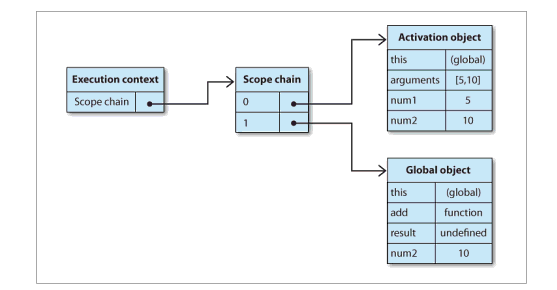
\includegraphics[width=1\textwidth]{figuras/scope_chain.png}
	\caption{Relación entre el contexto de ejecución y la \emph{scope chain}}
    \label{fig.scope_chain}
\end{figure}

Dentro de la función add, los identificadores \emph{num1} y \emph{num2} deben ser resueltos cuando la función esta ejecutando. Esta resolución se lleva a cabo inspeccionando
cada objeto en la \emph{scope chain} hasta que el identificador es encontrado. La búsqueda comienza con el primer elemento de la \emph{scope chain}, el cual es el registro
de activación que contiene las variables locales de la función. Si el identificador no es encontrado, el siguiente objeto de la \emph{scope chain} es inspeccionado en busca del
identificador.

Entender cómo funcionan los \emph{scopes} y las \emph{scope chain} en Javascript es importante, debido a que la performance de la resolución de identificadores esta directamente
relacionada al numero de objetos en la \emph{scope chain}.

\section{Variables locales}

Las variables locales son por lejos los identificadores más rápidos en los cuales se puede escribir y leer. Debido a que existen en los objetos de activación de la función
en ejecución, la resolución de identificadores involucra la inspección de un sólo objeto en la \emph{scope chain}. La cantidad de tiempo necesaria para leer el valor de una
variable aumenta con cada elemento que haya que inspeccionar en la \emph{scope chain}. Como las variables locales son las que se encuentran al comienzo de la \emph{scope chain}
son las mas rápidas de acceder, y por lo tanto es una buena práctica almacenar en variables locales todas las variables globales que sean referenciadas más de una vez
dentro de una función.

\section{La sentencia with}
La \emph{scope chain} para cierto contexto de ejecución normalmente no cambia durante la ejecución del código. Existen dos sentencias que temporalmente incrementan la
\emph{scope chain} de un contexto de ejecución. La primera es la sentencia with, que fue diseñada para permitir un acceso más simple a las propiedades de un objeto haciéndolas
parecer variables locales. Por ejemplo:

\begin{em}
var person = \{
    name: ``Nicholas'',
    age: 30
\};

function displayInfo()\{
    var count = 5;
    with(person)\{
        alert(name + `` is '' + age);
        alert(``Count is '' + count);
    \}
\}

displayInfo();
\end{em}

En esta función, el objeto \emph{person} es pasado en un bloque \emph{with}. Esto permite el acceso a las propiedades \emph{name} y \emph{age} como si hubieran sido definidas
de manera local. Lo que en verdad ocurre, es que un nuevo objeto es agregado al comienzo de la \emph{scope chain} del actual contexto de ejecucion.

\begin{figure}[h]
\centering
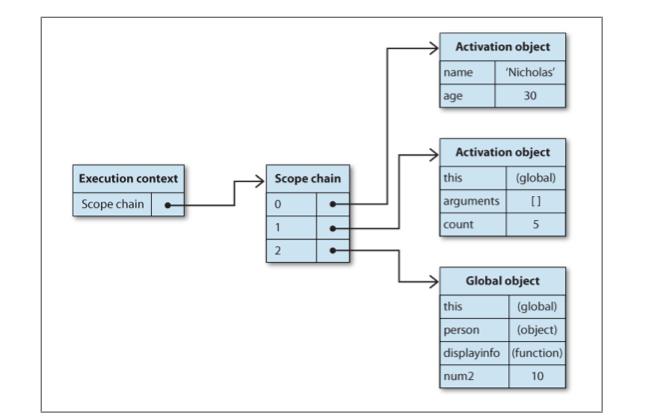
\includegraphics[width=1\textwidth]{figuras/scope_chain_with_statement.png}
	\caption{\emph{Scope chain} al utilizar la sentencia with}
    \label{fig.scope_chain_with_statement}
\end{figure}

Si bien el uso de esta sentencia puede parecer muy conveniente cuando las propiedades de un objeto son utilizadas con mucha frecuencia, este objeto extra en la
\emph{scope chain} del contexto daña la performance de la resolución de identificadores, debido a que las variables locales de la función pasan a encontrarse en el segundo
objeto en la \emph{scope chain}.

La sentencia \emph{catch} (correspondiente al bloque \emph{try catch}) es la segunda sentencia que aumenta el tamaño de la \emph{scope chain}. Ésta se comporta de manera
similar a la sentencia \emph{with} al agregar un objeto al comienzo de la \emph{scope chain} mientras ejecuta el código dentro del bloque. Ese objeto contiene una entrada
para la excepción especificada en la sentencia \emph{catch}. Sin embargo la sentencia \emph{catch} es ejecutada sólo cuando ocurre un error durante la ejecución de la
sentencia \emph{try}, resultando menos problemática que la snetencia \emph{with}.



\subsection{HTTP Caching}

EL protocolo HTTP es utilizado en sistemas de información distribuídos, donde la performance puede ser mejorada almacenando en cache las respuestas. La version 1.1 del
protocolo HTTP incluye un número de elementos destinados a mejorar el almacenamiento de elementos en cache.

El objetivo del \emph{caching} en HTTP/1.1 es eliminar la necesidad de enviar pedidos en algunos escenarios, y también evitar enviar respuestas completas en otros casos. Al evitar enviar algunos pedidos, se reduce el número de \emph{round-trips} requeridos para muchas operaciones (para ello se utiliza un mecanismo de expiración que se explicará más adelante). Por otro lado, al evitar el envío de respuestas completas se reducen los requerimientos de ancho de banda de la red.

Un concepto muy importante que hace posible el uso del cache es el de transparencia. La negociación transparente es una combinación de negociaciones del tipo \emph{server-driven}
y \emph{agent-driven}. Cuando un cache es suministrado con la lista de representaciones disponibles de las respuestas (como en negociaciones \emph{agent-driven}), y las
dimensiones de la varianza son completamente comprendidas por el cache, el mismo se vuelve capaz de realizar negociaciones \emph{server-driven} en nombre del servidor original
para subsiguientes pedidos de ese recurso.

\subsubsection{Correctitud del cache}
Un cache bien configurado debe responder a un pedido con la respuesta más actual mantenida en el cache, que sea apropiada al pedido recibido. La respuesta debe cumplir
con una de las siguientes condiciones.

\begin{enumerate}
  \item Fue comprobada su equivalencia con respecto a la respuesta que el servidor hubiera retornado, revalidando la misma con el servidor. El modelo de validación está definido
  en la sección 13.3 de \cite{rfc2616}, el cual es explicado más adelante en este documento.
  \item La respuesta es actual, lo cual implica que cumple con los requerimientos menos restrictivos del cliente, servidor y cache.
  Si la respuesta almacenada no es lo suficientemente actual según los requisitos tanto del cliente como del servidor, en circunstancias especiales un cache puede retornar
  la respuesta con el correspondiente encabezado \emph{Warning} definido en la seccion 13.1.2 de \cite{rfc2616}, a menos que la misma este prohibida, por ejemplo por una
  directiva \emph{``no store''} o \emph{``no-cache''}. Las mismas se encuentran definidas en la sección 14.9.2 de \cite{rfc2616} y serán examinadas más adelante en este
  documento.
  \item Es una respuesta apropiada del tipo 304 (Not Modified), 305 (Proxy Redirect), o de error (4xx or 5xx).
\end{enumerate}

Si un cache recibe una respuesta que normalmente enviaría al cliente (una respuesta completa o con estado 304), y la misma no es actual, el cache debería enviarsela
al cliente sin agregarle encabezados \emph{Warning}, pero sin removerlos en caso de que se encuentren presentes en la misma. Tampoco debería intentar revalidar una respuesta
simplemente porque la misma quedo desactualizada en el tránsito, debido a que esto puede ocasionar un loop infinito.

\subsubsection{Warnings}

Siempre que un cache retorne una respuesta que no es actual, debe agregar un encabezado \emph{Warning} a la misma. El encabezado \emph{Warning} y las advertencias son definidas
en la seccion 14.16 de \cite{rfc2612}. Este encabezado permite a los clientes tomar medidas apropiadas. El uso de \emph{Warnings} en vez de utilizar codigos de estado
de error es utilizado para distinguir estas respuestas de verdaderos casos de error.

Las \emph{Warnigns} tienen asignados codigos de advertencia de tres digitos. El primero indica si la \emph{Warning} debe o no ser eliminada de una entrada en cache despues de
una validacion exitosa.

\emph{Warnings} con codigo de estado 1xx describen el estado de actualidad o revalidacion de la respuesta, y por lo tanto deben ser eliminadas despues de una revalidacion
exitosa. Este tipo de \emph{Warning} pueden ser generadas por una cache solo cuando se intenta validar una entrada de la misma. No deben ser generadas por los clientes.
Por otro lado las \emph{Warnings} con codigo 2xx describen algun aspecto del cuerpo o de los encabezados de la respuesta que no fue rectificado por una revalidacion y que no
debe ser eliminado despues de una revalidacion exitosa.

Los caches en su version HTTP/1.0 almacenan todas las respuestas que contengan encabezados \emph{Warning}, sin eliminar los que tengan código en el rango 1xx. \emph{Warnings} en respuestas
que alcanzan caches de HTTP/1.0 contienen un campo extra (\emph{warning-date}), el cual previene que un receptor HTTP/1.1 malinterprete una \emph{Warning} que se encuentra en
cache de forma erronea.

\emph{Warnings} tambien contienen un texto de advertencia. El mismo puede estar en cualquier lenguaje natural, basado en los encabezados \emph{Accept} y, puede incluir un
indicador opcional del tipo de conjunto de caracteres que es utilizado. Multiples \emph{warnings} pueden ser adjuntadas a una respuesta, ya sea por el servidor de origen o
pir un cache, incluso pueden tener el mismo codigo. Por ejemplo un servidor pueder proveer la misma \emph{Warning} con el texto en diferentes idiomas.

Cuando una respuesta tiene multiples \emph{Warnings} asociadas, puede no ser practico desplegarle todas al usuario. La version 1.1 de HTTP no especifica reglas de prioridad
estrictas para determinar que \emph{Warnings} seran desplegadas al usuario ni en que orden.

\subsubsection{Mecanismos de \emph{cache-control}}

Los mecanismos basicos de cache en HTTP/1.1 consisten en especificar fechas de expiracion del lado del servidor y validadores, las cuales son directivas implicitas
para los caches. En algunos casos, un servidor o cliente puede necesitar proveer directivas explicitas a los caches de HTTP.
Para cumplir con este proposito se utlizan los encabezados \emph{Cache-Control}.

El encabezado \emph{Cache-Control} permite a un cliente o servidor transmitir una variedad de directivas tanto en pedidos como respuestas. Estas directivas tipicamente
sobreescriben los algoritmos de cache predeterminados. Como regla general, si existe un conflicto entre valores de encabezados, la interpretacion mas restrictiva es
aplicada. Las directivas de del encabezado \emph{Cache-Control} son descritas en detalle en la seccion 14.9 del \cite{rfc2616}.

\subsubsection{Modelo de expiracion}
\textbf{Server-Specified Expiration}

HTTP \emph{caching} funciona mejor cuando los caches pueden evitar completamente que se realicen pedidos al servidor de origen. El principal mecansimo para evitar esto, es que el servidor
de origen provea una fecha de expiracion explicita en el futuro, indicando que una respuesta puede ser utilizada para satisfacer pedidos posteriores. Se espera que los
servidores asignen fechas de expiracion futuras a las respuestas, con la creencia de que es poco probable que la entidad cambie antes que la fecha de expiracion sea alcanzada.
Los mecanismos de expiracion aplican solo a respuestas obtenidas de un cache y no a primeras respuestas, las cuales son enviadas de forma inmediata al cliente.

Si un servidor servidor desea forzar que una cache HTTP/1.1 valide cada pedido, sin importar como este configurada debe utilizar la directiva \emph{must-revalidate}.
Los servidores especifican fechas de expiracion explicitas utilizando el encabezado \emph{Expires} o la directiva \emph{max-age} del encabezado \emph{Cache-Control}.

\textbf{Expiracion heuristica}
Debido a que los servidores no siempre proveen fechas de expiracion explicitas, los caches tipicamente asignan fechas de expiracion aplicando heuristicas, empleando
algoritmos que utilizan los valores de otros encabezados (como los del \emph{Last-Modified}) para estimar una fecha de expiracion plausible.

\subsection{Modelo de validacion}
Cuando un cache tiene una entrada no muy actual que desea usar como respuesta a un pedido de un cliente, primero tiene que comprobar con el servidor de origen
(o posiblemente con un cache intermedio que contenga una respuesta actual) si la respuesta es valida. Esto se denomina validar la entrada del cache. Como no se quiere tener el overhead
de retransmitir la respuesta completa en caso de que la respuesta sea valida, y tampoco tener el overhead de un \emph{round-trip} extra en caso de que la entrada sea
invalida, HTTP/1.1 soporta el uso de pedidos condicionales.

La clave para soportar pedidos condicionales son los denominados validadores de cache. Cuando un servidor genera una respuesta completa, adjunta un validador a la misma,
el cual es almacenado como parte de la entrada en el cache. Por otro lado cuando un cliente realiza un pedido condicional por un recurso para el cual tiene una entrada
en su cache, incluye el validador en el pedido.

El servidor luego verifica el validador presente en el pedido con el correspondiente a la entidad, y en caso de coincidir, retorna una respuesta con codigo 304
y sin cuerpo. En otro caso retorna una respuesta completa. En consecuencia se evita transmitir la respuesta completa si los validadores coniciden y se evita un \emph{round trip}
extra en caso contrario.

A continuacion se nombran algunos validadores.

\subsubsection{Last-Modified Dates}
El valor del encabezado \emph{Last-Modified} es utilizado como validador (especificado en el rfc 2616 \cite{rfc2616} sección 14.29). Una entrada de una cache puede ser
considerada valida si la entidad no ha sido modificada desde el valor contenido en este encabezado.

\subsubsection{Entity Tag}
El encabezado \emph{ETag} (definido en la seccion 14.19 de \cite{rfc2616}), es un tipo de validador. Permite una validacion mas confiable en situaciones en las cuales es inconveniente almacenar
fechas de modificacion, donde la resolucion \emph{one-second} de fechas de HTTP no es suficiente o donde el servidor de origen desea evitar ciertas paradojas que pueden surgir por el uso de
fechas de modificacion.

\subsubsection{Validadores fuertes y debiles}
Tanto el servidor de origen como los caches comparan dos validadores para decidir si representan la misma entidad, es normal esperar que si una entidad cambia en algun
sentido, el validador asociador tambien lo haga. Este es el caso de los validadores fuertes.
Sin embargo, existen casos en los que un servidor prefiere cambiar los validadores solo si existen cambios semanticos significativos, y no cuando cambian aspectos menores
de una entidad. Un validador que no siempre cambia cuando la entidad asociada lo hace es conocido como un validador debil.
Se puede ver un validador fuerte como uno que cambia cada vez que cambia un bit de la entidad asociada, mientras que uno debil cambia solo cuando el significado de la
entidad asociada cambia.
Un validador es utilizado o bien cuando un cliente genera un pedido e incluye el validador en un encabezado, o bien cuando un servidor compara dos validadores.

Los validadores fuertes son utilizables en cualquier contexto, mientras que los debiles son utilizables en contextos en los cuales no se depende de la exactitud de una entidad.
Por ejemplo, ambos pueden utilizarse para un pedido condicional de una entidad completa. Sin embargo, solo los validadores fuertes pueden utilizarse en un pedido parcial
de una entidad, a que de lo contrario el cliente puede terminar con una entidad inconsistente.

La unica funcion que el protocolo HTTP/1.1 define para los validadores es la comparacion. Existen dos funciones para comparar validadores, dependiendo de si el contexto
de la comparacion permte el uso de validadores debiles o no.

La funcion de comparacion fuerte, considera dos validadores como iguales si ambos son identicos en todo sentido y los dos son validadores fuertes. En cambio, la funcion de
comparacion debil considera dos validadores como iguales si ambos son identicos, pero uno de los dos es debil.

El comportamiento recomendado por el rfc 2616 \cite{rfc2616} para un servidor HTTP/1.1 es enviar una respuesta con una \emph{entity tag} fuerte (comportamiento por defecto)
y un encabezado \emph{Last-Modified}. Segun la especificacion un servidor al recibir un pedido condicional que incluye un encabezado \emph{Last-Modified} y una o mas
\emph{entity tags} como validadores no debe retornar una respuesta con estado 304, a menos que sea consistente con todos los campos de los encabezados en el pedido.
En el mismo escenario Un \emph{caching proxy} HTTP/1.1, no debe retornar al cliente una respuesta almacenada en su cache local a menos que la misma sea consistente con todos
los campos de los encabezados condicionales del pedido.

\subsection{Revalidacion de cache}
Algunas veces un \emph{user-agent} necesitar insistir que un cache revalide una entrada en su cache con el servidor de origen (y no con el siguiente cache que se encuentra
en el camino entre el y el servidor de origen) o recargar una entrada en su cache con el servidor de origen. Revalidaciones \emph{End-toEnd} pueden ser necesarias si tanto el
cache como el servidor de origen sobreestiman la fecha de expiracion de la respuesta almacenada en el cache. La recarga puede ser necesaria si la entrada de la cache ha sido
corrompida por algun motivo.

La revalidacion \emph{End-to-End} puede ser pedida cuando el cliente no tiene una copia local en su cache, en cuyo caso es denominada \emph{unspecified end-to-end revalidation}
o cuando un cliente tiene una copia local almacenada en su cache, en cuyo caso se denomina \emph{specific end-to-end revalidation}.

El cliente puede especificar tres tipos de acciones utilizando las directivas de \emph{Cache-Control}: \emph{end-to-end reload}, \emph{Specific end-to-end revalidation} y
\emph{Unspecified end-to-end revalidation}.
En la accion \emph{End-to-end reload}, el pedido incluye la directiva \emph{no-cache} o por compatibilidad con la version anterior del protocolo \emph{Pragma: no-cache}.
\emph{Field-names} no deben incluirse con esta directiva en un pedido, y el servidor no debe utilizar una capia en cache para responder a este pedido.
En cambio \emph{Specific end-to-end revalidation} incluye la directiva \emph{max-age=0}, la cual fuerza que cada cache en el camino entre el cliente y el servidor de origen
revalide su propia entrada con el siguiente cache o servidor. El pedido inicial incluye un validador condicional con el validador actual del cliente.
Por ultimo la accion \emph{Unspecified end-to-end revalidation} tambien fuerza a que los caches que se encuentran en el camino entre el cliente y el servidor de origen
revaliden su entrada con el siguiente cache o servidor. El pedido inicial no incluye un validador condicional, si lo incluye el primer cache en el camino (en caso de existirlo)
que contenga una entrada para ese recurso en particular.



\chapter{Selectores de CSS}
Entender como los navegadores parsean las reglas de estilo y renderizan las páginas web es una tarea importante al momento de mejorar la performance de una página web.
A medida que los navegadores parsean el documento HTML, construyen una estructura arborescente que representa todos los elementos que van a ser desplegados en la página.
Una vez completa esta etapa, busca las reglas que aplican a los elementos en diversas hojas de estilo, de acuerdo a las reglas de cascada, herencia y orden de CSS.

En la mayoría de las implementaciones de los navegadores, el motor de CSS busca reglas en las hojas de estilo que aplican a cada elemento del documento, evaluándolas de derecha a izquierda 
(debido a que el parser que utilizan es \emph{bottom-up}), empezando por el selector de más a la derecha, conocido como \emph{key} y
moviendose a través del selector hasta encontrar una concordancia o descartando la regla en otro caso.

En base a este sistema, mientras menos reglas tengan que ser evaludas por el motor de estilos, mejor será la performance del mismo. Por lo tanto remover reglas que no aplican es
un paso importante para mejorar la performance del renderizado, pero aún más importante es optimizar las definiciones de las reglas. Un aspecto clave al optimizar
las reglas de estilo, es definir reglas para que sean lo mas específicas posible y evitar redundancia en las mismas, para que de esta forma el motor de estilos pueda
encontrar rápidamente concordancias, evitando perder tiempo evaluando reglas que no aplican.

\section{Tipos de selectores}
En esta sección se listan los distintos tipos de selectores de CSS ordenados en base al costo en cuanto a la performance de los mismos, comenzando por los que tienen
menor impacto en la performance al momento de aplicar las reglas.

\subsection{Id}
Simple y eficiente, este selector aplica al único elemento en el documento HTML cuyo atributo \emph{ID} coincida con el de la regla.

\subsection{Clase}
Las reglas basadas en clases, se especifican con un punto seguido por el nombre de la clase. Los selectores de clase se aplican a todos los elementos que contengan la clase
de la regla en su atributo clase.

\subsection{Tipo}
Los selectores de tipo aplican a todos los elementos de un tipo especifico. La regla \emph{a\{text-decoration: none;\}} remueve el subrayado del texto de todos los
\emph{anchors} que se encuentren en la página. El uso de estas reglases una forma eficiente de agregar estilos a todos los elementos de un tipo especifico sin tener que
agregar caracteres extra, como clases a los elementos.

\subsection{Hermano adyacente}
Este selector consiste en concatenar dos selectores mediante el simbolo +. La regla \emph{h1 + \#toc} aplica al elemento que tiene \emph{toc} como atributo \emph{ID}, cuyo
hermano previo es un elemento del tipo \emph{h1}.

\subsection{Hijo \emph{child}}
Este tipo de selector es formado por la combinacion de dos o mas selectores simples mediante el uso del símbolo \emph{\textgreater}. La regla \emph{\#toc \textgreater   li \{font-weight: bold;\}}
aplica a todos los elementos del tipo \emph{li}, cuyo padre es el elemento con el atributo \emph{ID} igual a toc.

\subsection{Descendiente}
Estos selectores utilizan un espacio \emph{' '} como combinador. La siguiente regla \emph{\#toc a \{ color: \#444\}}, aplica a todos los elementos del tipo \emph{a} que sean
descendientes de el elemento cuyo \emph{ID} es igual a toc.

\subsection{Universales}
Los selectores universales (reglas representadas con un *) aplican a todos los elementos del documento.

\subsection{Atributo}
Los selectores por atributo aplican basandose en la existencia o valor de los atributos de un elemento. Un ejemplo de esto es la siguiente regla
\emph{[href='\#index'] \{font-style: italic;\}}.

\subsection{Pseudo-Clase y Pseudo-Elementos}
Este tipo de selectores son utilizados para aplicar a situaciones en las cuales la información no esta representada en el DOM. Algunas de las \emph{pseudo-classes} más
utilizadas son :hover, :visited, :first-child, :focus, etc.

\section{Reglas a evitar}

\subsection{No sobrecargar los selectores por Id}
Debido a que existe un único elemento en la página con un id específico, no es necesario agregar clasificadores extra ya que la única consecuencia que tiene esto es
retrasar el proceso. Por lo que es recomendable evitar reglas del estilo \emph{div\#toc}.

\subsection{No sobrecargar selectores de clase}
En vez de clasificar selectores de clase para etiquetas específicas, se recomienda extender el nombre de la clase para que sea específico con el caso de uso que se quiere
tratar. Por ejemplo, si se tiene una regla de este tipo \emph{li.chapter}, se recomienda cambiarla por \emph{.li-chapter} o mejor aun \emph{.list-chapter}.

\subsection{Reglas especificas}
La principal causa de la disminución de la eficiencia de la aplicación de los selectores es la existencia de múltiples etiquetas en una regla. Es mejor dividir estos
selectores en clases y agregarlas a los elementos correspondientes. Por ejemplo, es recomendable cambiar las reglas del tipo \emph{ol li a} por selectores de clases
del tipo \emph{.list-anchor}.

\subsection{Evitar selectores de descendencia y \emph{child}}
Los selectores por descendencia son los más costosos de procesar, debido a que por cada elemento que aplica a cada parte de la regla se debe evaluar otro nodo más. En
vez de estos es mejor utilizar clases asociadas a los elementos de la regla.

\subsection{Utilizar herencia de los atributos}
Muchas de las reglas de CSS se heredan, es mucho más costoso especificar este tipo de propiedades en cada elemento a tenerlas en un ancestro del mismo del cual
pueden heredarlas.

\end{comment}

